\documentclass[a4]{article}
\usepackage{geometry}
\geometry{a4paper,left=2cm,right=3cm, top=2cm, bottom=2cm} 
%\usepackage[austrian]{babel}
\renewcommand{\familydefault}{\sfdefault}
\usepackage{amsfonts,latexsym,amssymb,graphicx}
\usepackage{subfigure,epsfig,epstopdf}
%\usepackage{pdfsync}
\usepackage[utf8]{inputenc}
%\usepackage[T1]{fontenc}
\usepackage{booktabs} % For professional looking tables
\usepackage{multirow}
\title{\bf 183.605 \\ Machine Learning for Visual Computing \\ Assignment 1}
\author{Group 12: \\
	Hanna Huber (0925230) \\ Lena Trautmann (1526567) \\ Elisabeth Wetzer ()}
\date{\today}


\begin{document}
\maketitle
\noindent

\begin{itemize}
\item Upload a zip-file with the required programs. You can choose the programming language.
\item Add a PDF document with answers to all of the questions of the assignment (particularly all required plots) and description and discussion of results. 
\end{itemize}

\section{Assignment 1}
\subsection{Part 1: Binary classification and the perceptron}

\subsubsection{Reading data}\label{sec:readdata}
\noindent {\bf Tasks:}
\begin{itemize}
\item Read the data using functions of your programming language resp. simulation software.
\end{itemize}
First, we wrote a new .csv-file with our .py-script to delete all extra blanks. Afterwards we could read in the data using \texttt{dlmread()}.

\begin{itemize}
\item Plot the input vectors in $\mathbb{R}^2$ and visualize corresponding target values (e.g. by using color). 
\end{itemize}
\begin{figure}[!h]
	\begin{center}
		\centering
		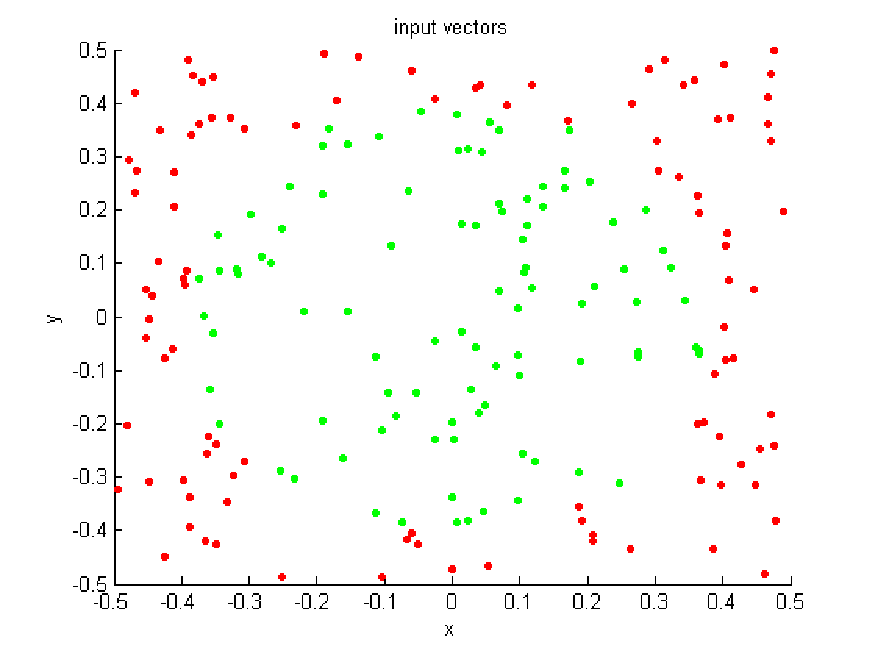
\includegraphics[width=6cm]{../figures/inputVectors.pdf}
	\end{center}	
	\caption{Plot of the input vectors with the target value visualized by colour.}
	\label{fig:inputVectors}
\end{figure}
Fig.~\ref{fig:inputVectors} shows the input vectors.

\begin{itemize}
\item Use the feature transformation $(x_1,x_2) \rightarrow (x_1^2,x_2^2)$ and plot the data in the new feature space. The data should now be linearly separable.
\end{itemize}
\begin{figure}[!h]
	\begin{center}
		\centering
		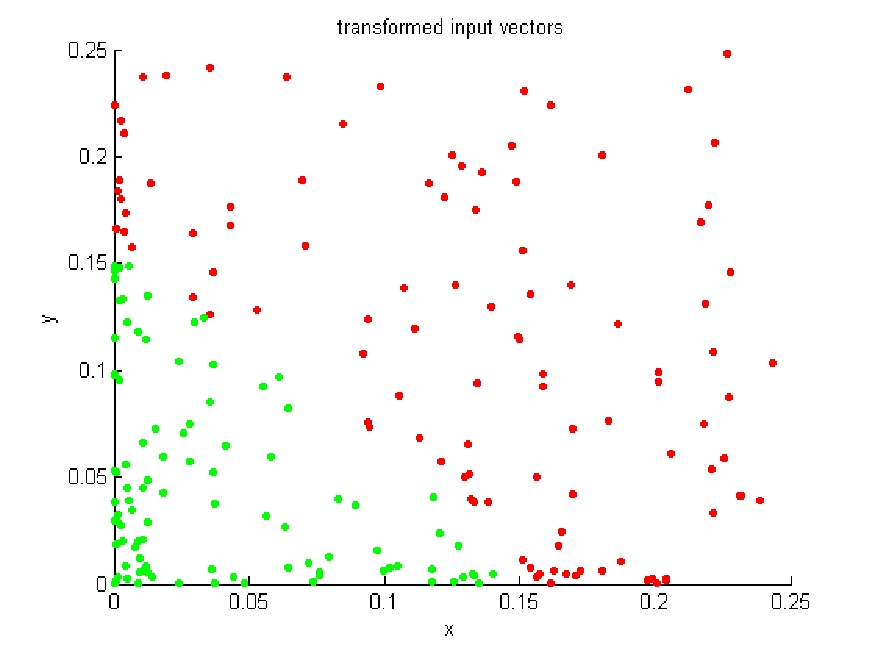
\includegraphics[width=6cm]{../figures/transformedInputVectors.pdf}
	\end{center}
	\caption{Plot of the transformed input vectors with the target value visualized by colour.}
	\label{fig:transformedInputVectors}
\end{figure}
Fig.~\ref{fig:transformedInputVectors} shows the transformed input vectors.

\subsubsection{Perceptron training algorithm}
The function
\begin{center}
\texttt{y = perc(w,X)}.
\end{center}
simulates a perceptron. The first argument is the weight vector ${\bf w}$ and the second argument is a matrix with input vectors in its columns ${\bf X}$. The output ${\bf y}$ is a binary vector with class labels 1 or -1.

The function 
\begin{center}
\texttt{w = percTrain(X,t,maxIts,online)}.
\end{center} 
returns a weight vector ${\bf w}$ corresponding to the decision boundary separating the input vectors in ${\bf X}$ according to their target values ${\bf t}$.

The argument $\texttt{maxIts}$ determines an upper limit for iterations of the gradient based optimization procedure. If this upper limit is reached before a solution vector is found, the function returns the current ${\bf w}$, otherwise it returns the solution weight vector. \texttt{online} is \emph{true} if the \emph{online}-version of the optimization procedure is to be used or \emph{false} for the \emph{batch}-version. 
\vspace{2mm}

\noindent {\bf Tasks:}
\begin{itemize}
\item The functions \texttt{percTrain} and \texttt{perc} are implemented in the files \texttt{percTrain.m} and \texttt{perc.m}, respectively.

\item Figures~\ref{fig:origOL},~\ref{fig:transOL},~\ref{fig:origBA},~\ref{fig:transBA} show perceptron learning after the first iteration, half of the iterations needed and after the final iteration. They show that the algorithm converges much faster using online learning (see Figures~\ref{fig:origOL} and~\ref{fig:transOL}). Figures~\ref{fig:transOL} and~\ref{fig:transBA} illustrate how the transformation into the feature space of basis functions makes the data linearly separable. The non-linear decision boundary in the original data space is obtained by applying the inverse transformation to the linear decision boundary in feature space.
\begin{figure}[h!]
\centering
	\subfigure[]{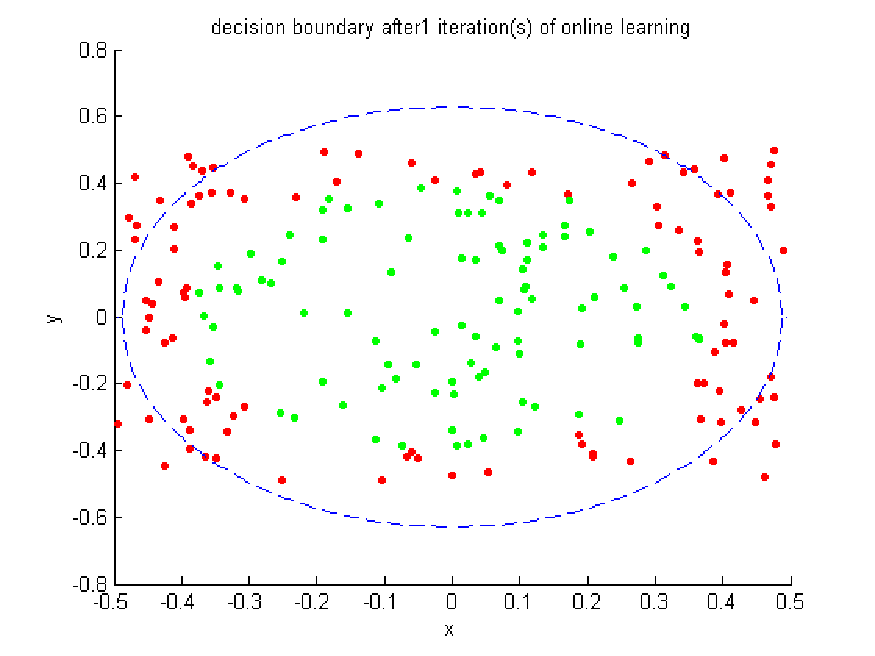
\includegraphics[width=5cm]{../figures/originalOnlineIt1.pdf}}
	\subfigure[]{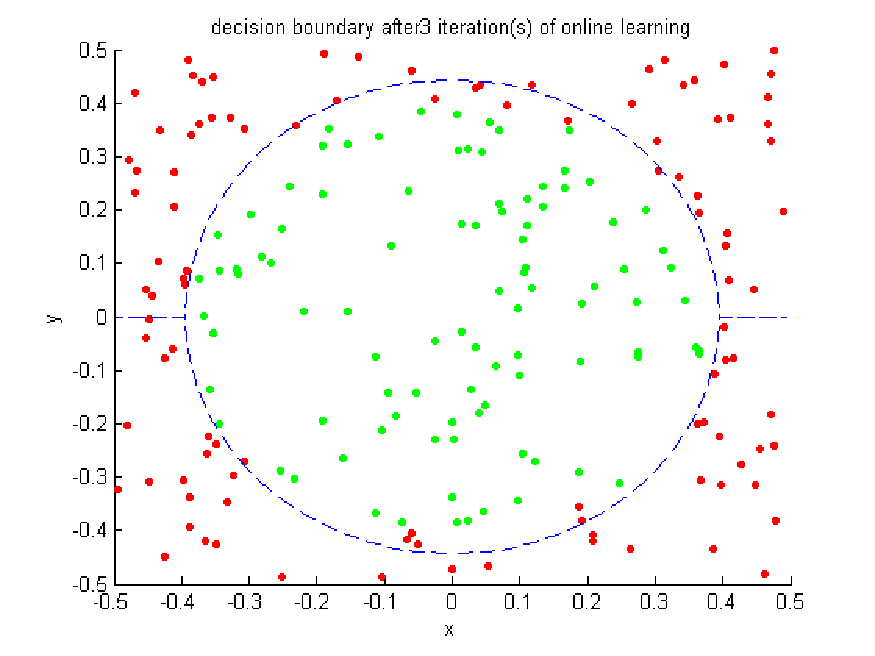
\includegraphics[width=5cm]{../figures/originalOnlineIt3.pdf}}
	\subfigure[]{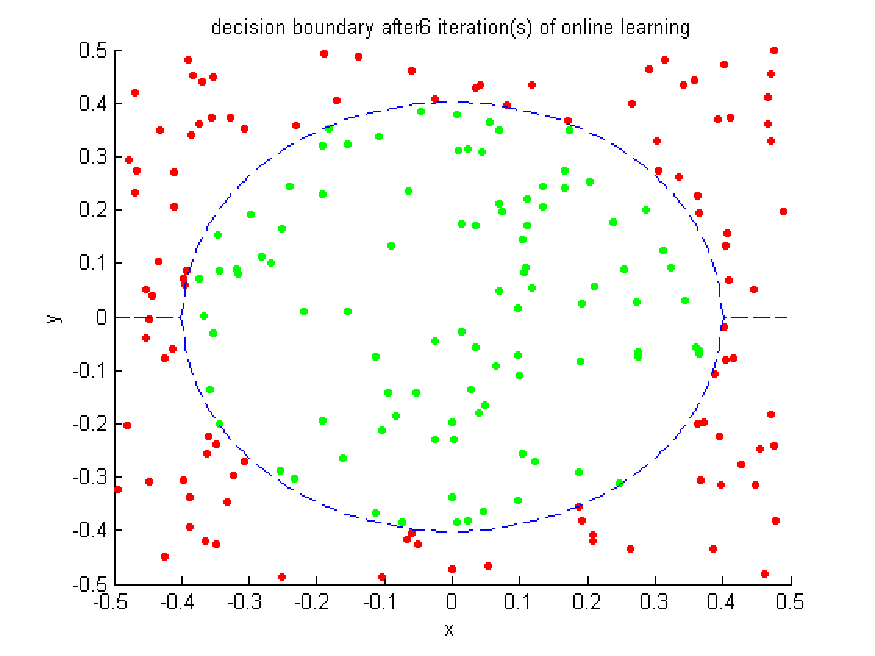
\includegraphics[width=5cm]{../figures/originalOnlineIt6.pdf}}
\caption{Perceptron decision boundary in the original data space at iterations \#1, \#3 and \#6 of online learning.}
\label{fig:origOL}
\end{figure}
\begin{figure}[h!]
\centering
	\subfigure[]{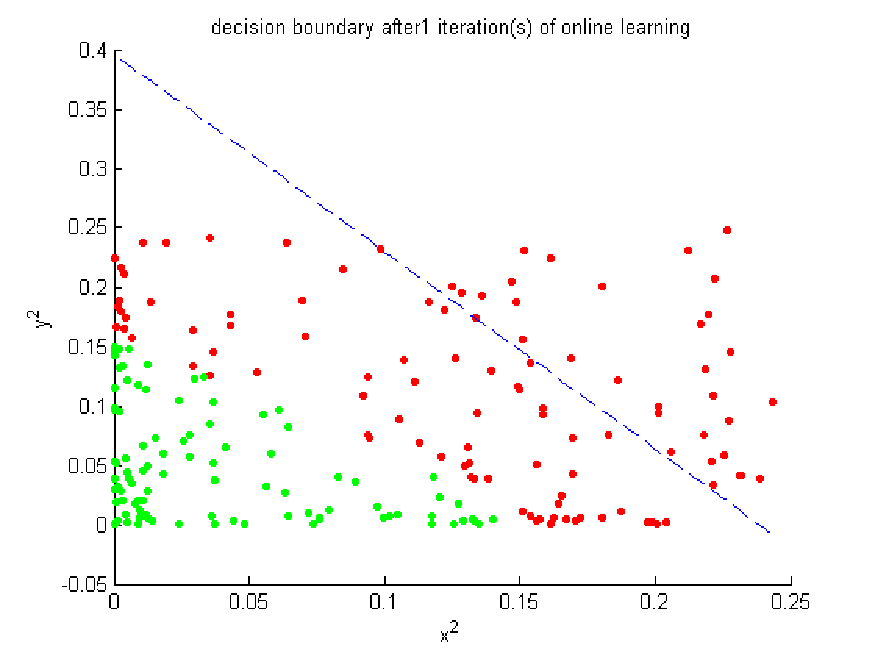
\includegraphics[width=5cm]{../figures/transformedOnlineIt1.pdf}}
	\subfigure[]{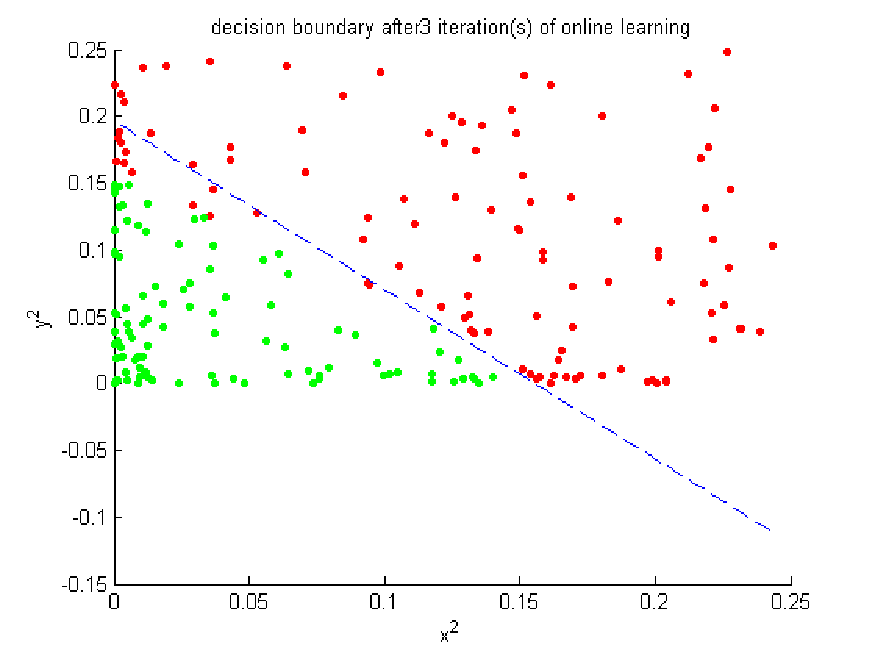
\includegraphics[width=5cm]{../figures/transformedOnlineIt3.pdf}}
	\subfigure[]{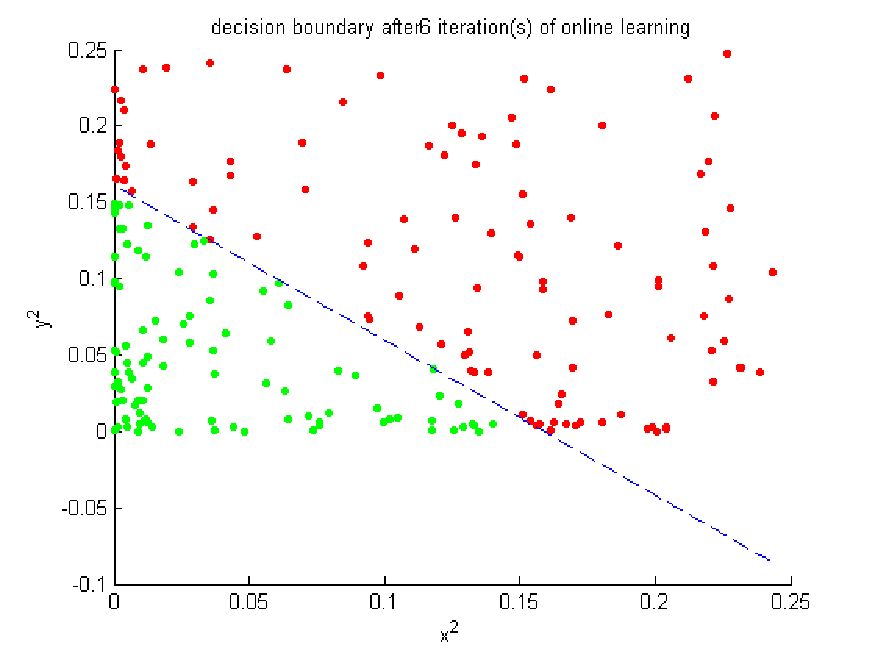
\includegraphics[width=5cm]{../figures/transformedOnlineIt6.pdf}}
\caption{Perceptron decision boundary in the feature space of basis functions at iterations \#1, \#3 and \#6 of online learning.}
\label{fig:transOL}
\end{figure}
\begin{figure}[h!]
\centering
	\subfigure[]{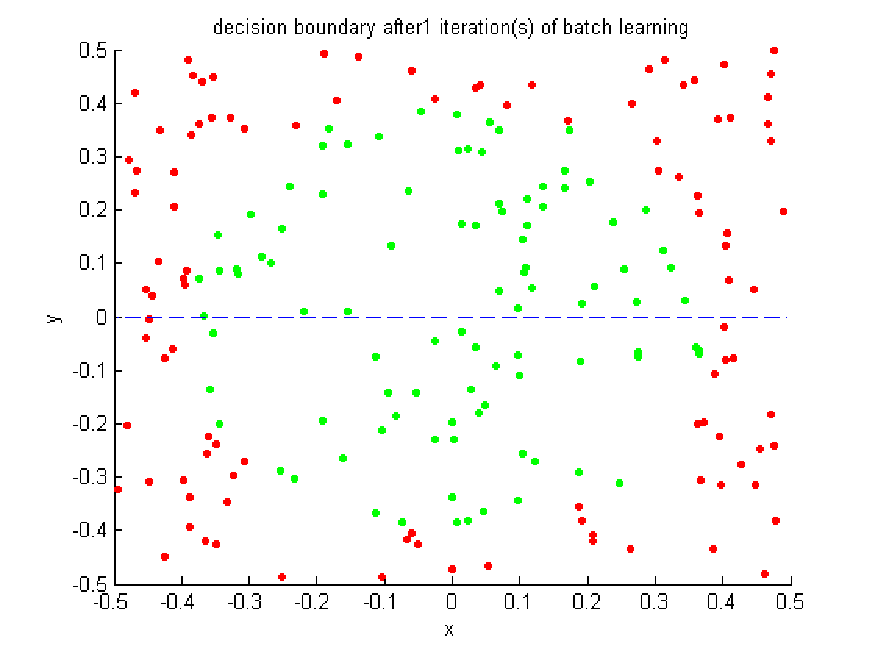
\includegraphics[width=5cm]{../figures/originalBatchIt1.pdf}}
	\subfigure[]{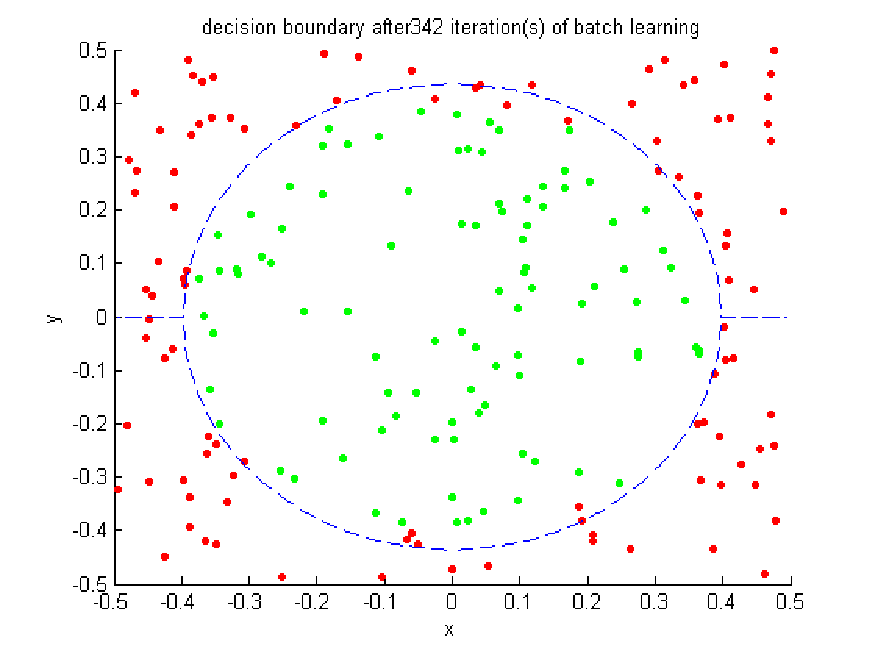
\includegraphics[width=5cm]{../figures/originalBatchIt342.pdf}}
	\subfigure[]{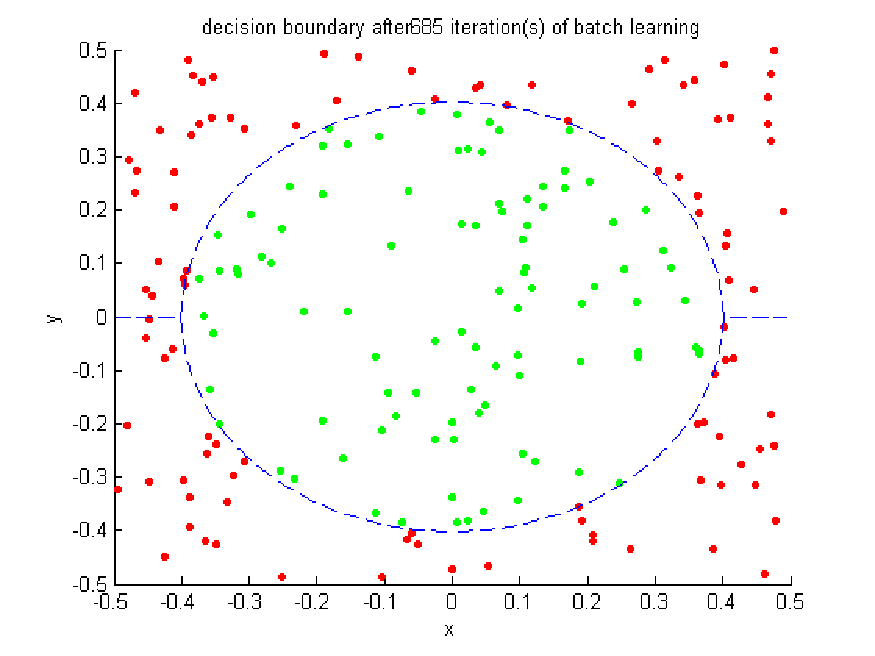
\includegraphics[width=5cm]{../figures/originalBatchIt685.pdf}}
\caption{Perceptron decision boundary in the original data space at iterations \#1, \#342 and \#685 of batch learning.}
\label{fig:origBA}
\end{figure}
\begin{figure}[h!]
\centering
	\subfigure[]{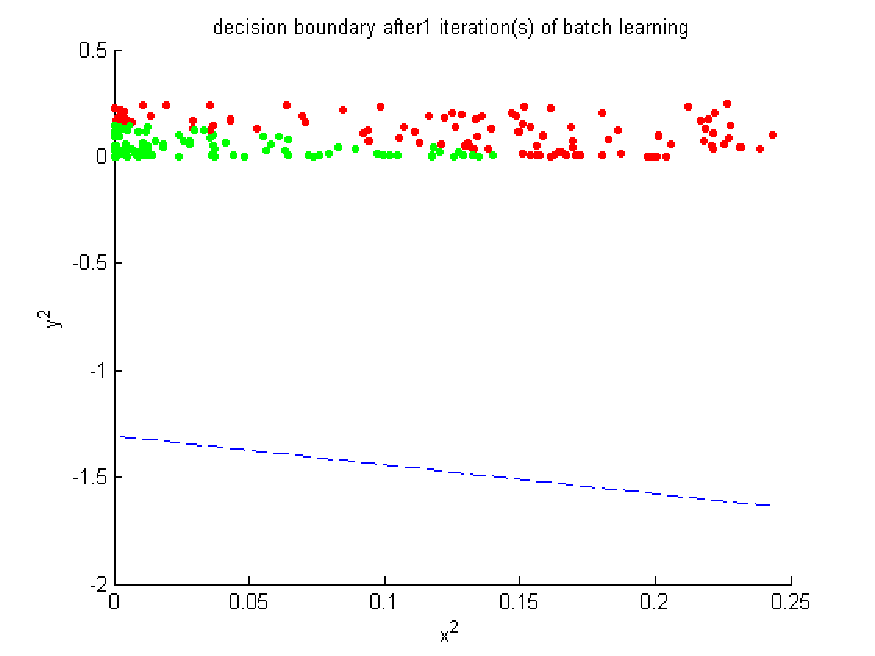
\includegraphics[width=5cm]{../figures/transformedBatchIt1.pdf}}
	\subfigure[]{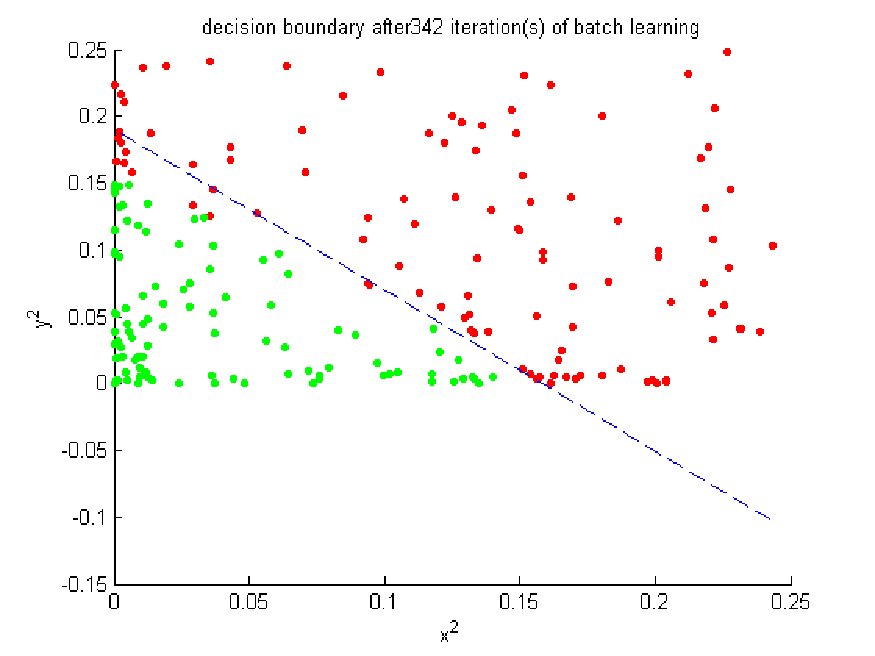
\includegraphics[width=5cm]{../figures/transformedBatchIt342.pdf}}
	\subfigure[]{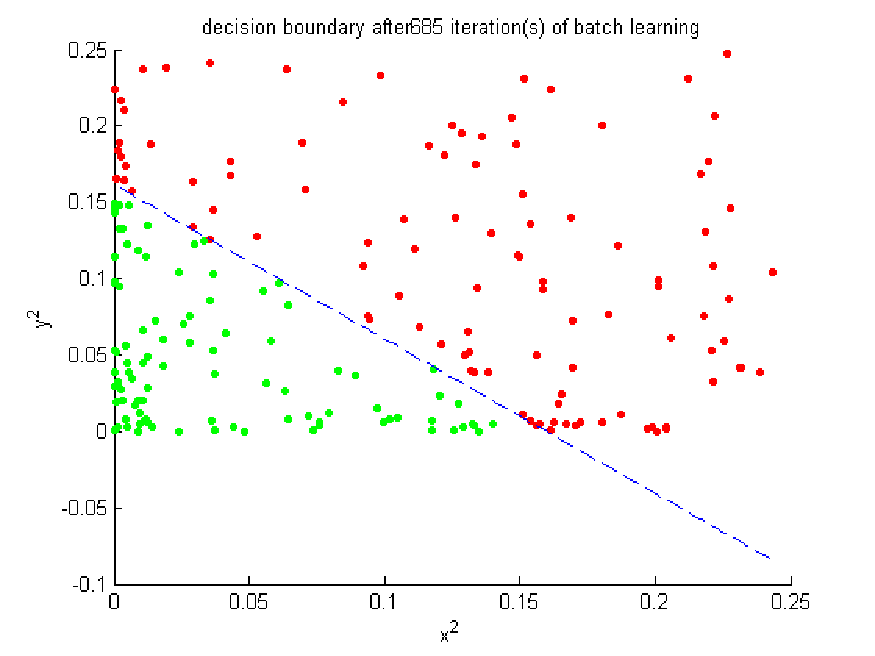
\includegraphics[width=5cm]{../figures/transformedBatchIt685.pdf}}
\caption{Perceptron decision boundary in the feature space of basis functions at iterations \#1, \#342 and \#685 of batch learning.}
\label{fig:transBA}
\end{figure}
\item The weight vector is initialized as ${\bf w} = {\bf 0}$. This way, the learning rate $\gamma$ merely scales the weight vector ${\bf w^{(j)}} = \gamma \sum_{i\in M}x_it_i$, where $j$ denotes the current iteration and $M$ the set of data points that have been misclassified and used to update {\bf w} up to this point. As $(\gamma_1 \sum_{i\in M}x_it_i)^T (x_kt_k) \leq 0 \Leftrightarrow  (\gamma_2 \sum_{i\in M}x_it_i)^T (x_kt_k) \leq 0$ for any $\gamma_1, \gamma_2 > 0$, the classification of the $k$th data point and thus the learning behaviour of the perceptron are not influenced by the learning rate.
\end{itemize}

\begin{figure}[!h]
\begin{center}
\centering
	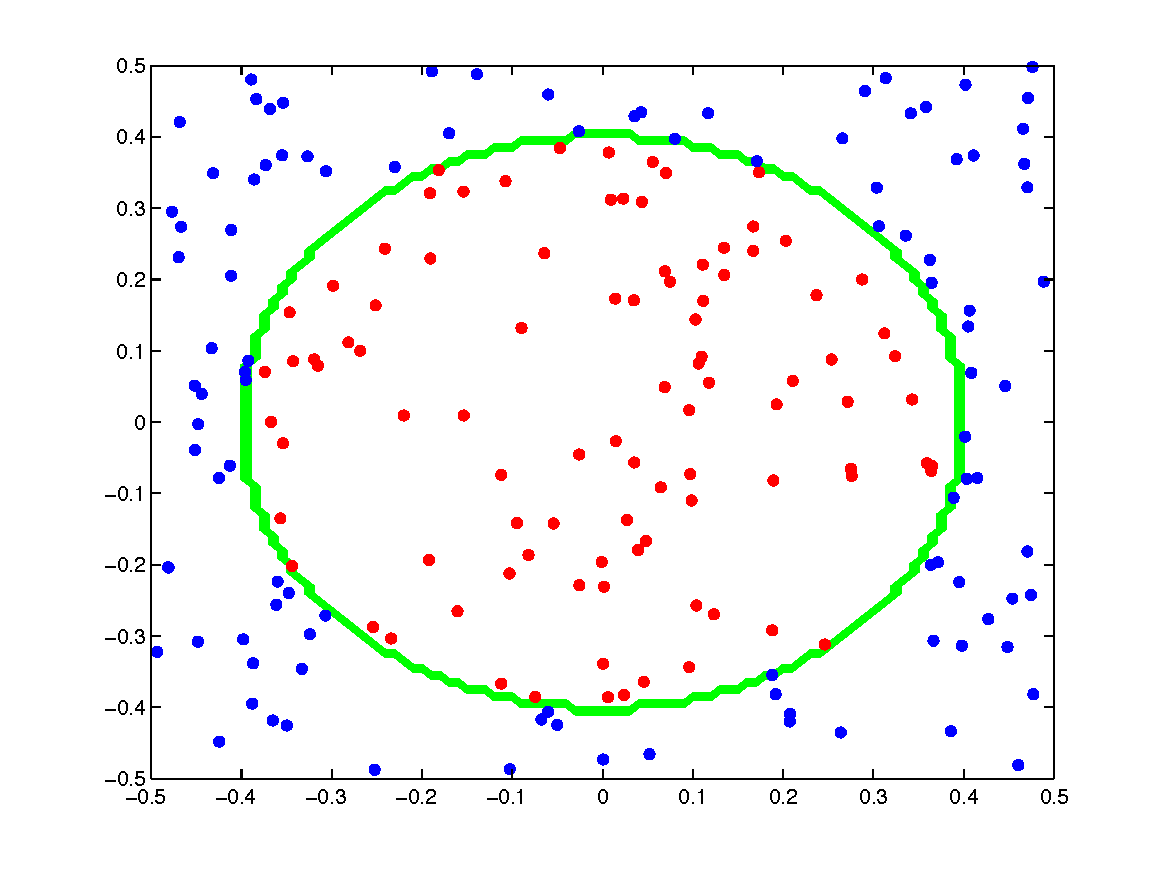
\includegraphics[width=6cm]{../figures/perceptron.pdf}
\end{center}
\caption{\label{fig:perceptron}Plot of the decision boundary in the original data space found by the perceptron (green curve) together with labelled data points.}
\end{figure}

\subsection{Part 2: Linear basis function models for regression}

%Aim of this exercise to deepen understanding of parameter optimization of error function while taking into account the relation of model complexity (in this case it corresponds to the number of basis functions used) and the expected error. Since this expected value (the mean squared error) is a theoretical quantity, it has to be estimated by the average of the error of predictions resulting from many training runs with different randomly generated target values.

\subsubsection{Experimental setup}
%A row vector of scalar inputs $x \in [0,5]$ sampling the interval in steps of $0.1$ (resulting in 51 values) and a corresponding output vector $\mathbf{y}$ with values $y = f(x) = 2x^2-Gx+1$ is the basis of this experiment. The coefficient $G$ is your group number. These 51 points are to be used for the visualization of the target function and the predictions of the fitted model.
%A training set is generated by subsampling the 51 values as follows: Every eighth value ($x_0 = 0$, $x_1 = 0.8$, $x_2 = 0.16$, ...) is assigned to the training set and the target values $t_i$ are obtained by adding to the corresponding $y_i$ a random value from the normal distribution $\mathcal{N}(\mu = 0,\sigma = 16)$. Thus, the training set contains $N = 9$ pairs of observations $x_i, t_i$. 
%
%We will employ a linear basis function model of the form $f_{\mathbf w}(x) = {\mathbf w}^T{\mathbf \Phi}(x)$, where\begin{equation} \nonumber
%{\mathbf \Phi}(x) \rightarrow \left(
%\begin{array}{c} 1\\ x \\ x^2 \\ \vdots \\ x^d \\ \end{array}\right),
%\end{equation} 
%and ${\mathbf w} \in \mathbb{R}^{d+1}$. The model will be fitted to the training set by minimization of the training error 
%\begin{equation}
%E({\mathbf w}) = \sum_{i = 1}^N(t_i - {\mathbf w}^T{\mathbf \Phi}(x_i))^2
%\end{equation} 
%also known as the \emph{residual sum of squares} (RSS). The optimal weight vector is given by ${\mathbf w}^* = \arg\min_{\mathbf w} E({\mathbf w})$.
%
%
%\begin{figure}[!h]
%\begin{center}
%\centering
%	\subfigure[]{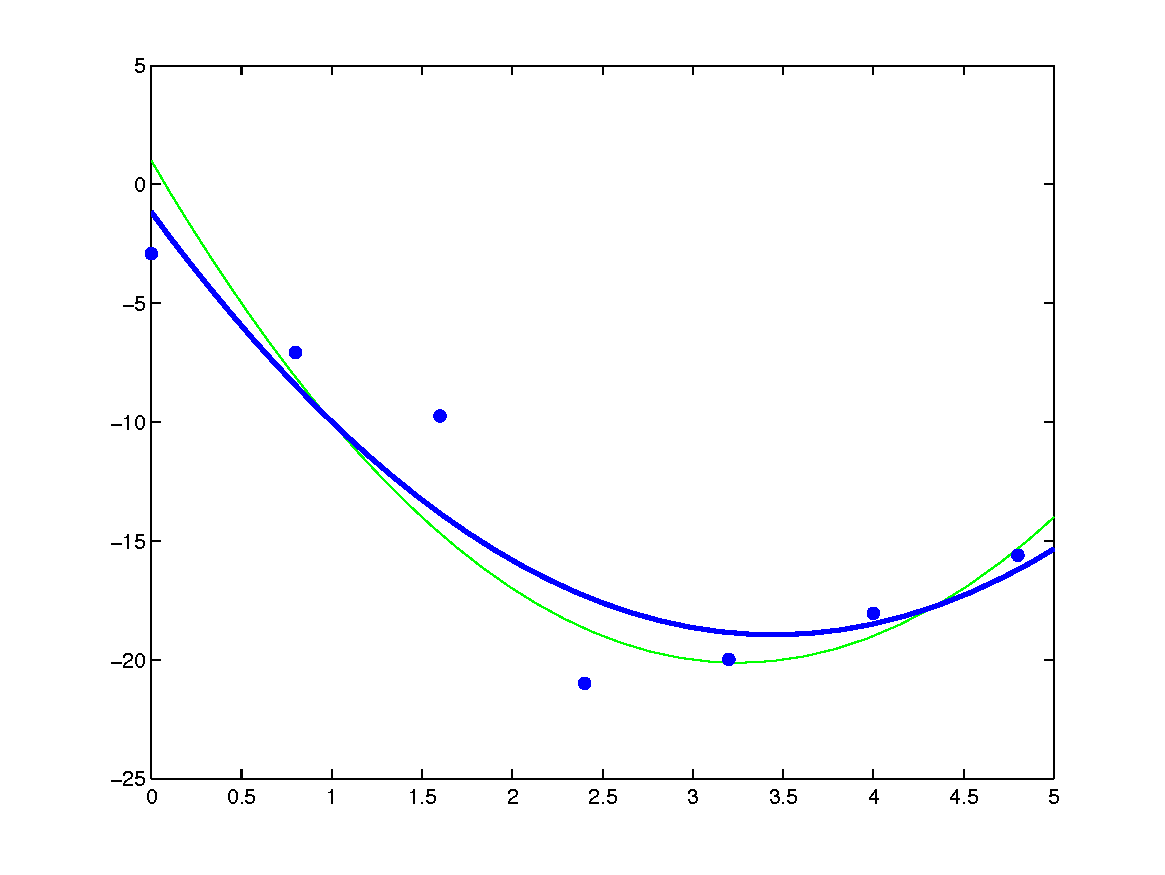
\includegraphics[width=5.5cm]{../figures/regressiond2.pdf}}
%	\subfigure[]{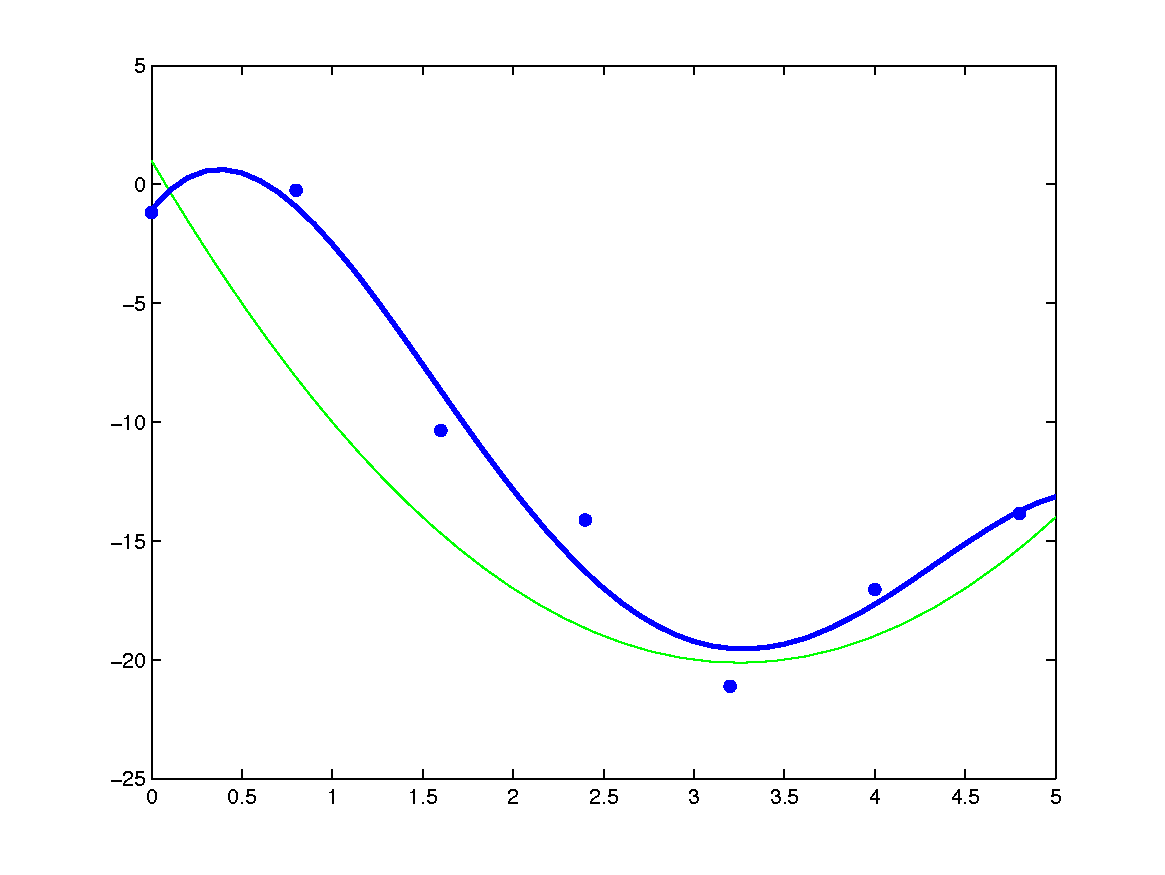
\includegraphics[width=5.5cm]{../figures/regressiond4.pdf}}
%\end{center}
%\caption{An example of a true target function (thin green curve) from which the training data was generated, training set (without feature transformation) with $N=9$ (blue dots) and prediction of the fitted model ${\mathbf w}^T{\mathbf \Phi}(x)$ (blue curve). The basis functions are ${\mathbf \Phi}(x) \rightarrow (1,x,x^2,x^3,...,x^d)^T$. (a) $d=2$ (b) $d=4$.}
%\end{figure}
At the end of the setup we have:
\begin{itemize}
	\item xtrain and ttrain: the training data
	\item phi: the transformation function
	\item xtrain\_phi: the transformation of xtrain
\end{itemize} 

\subsubsection{Optimization: \emph{LMS}-learning rule vs. closed form}
%
%Use a linear unit (\emph{online} LMS-learning rule) for regression on transformed input data. In a first step use a linear basis function model with $d=2$ (in Matlab you can calculate the power elementwise: e.g. \texttt{[x x x].$\wedge$ [0 1 2]}). Hint: Visualize $y$ and its prediction during the training or observe the chance of the weight vector to determine useful values for $\gamma$.
%\vspace{2mm}
%
\noindent {\bf Tasks:}
\begin{itemize}
	\item What is the resulting weight vector when using the LMS-rule?
\end{itemize}
\begin{table} [tbp!]
	\caption{Weight vector derived for the LMS-rule and of closed form}
	\centering
	\label{table:wLMS}
	\begin{tabular}{l c c c}
		\toprule
		& $\phi_0$ & $\phi_1$ & $\phi_2$ \\ 
		\midrule
%		wLMS & 0.7191 & -10.8810 & 1.6695 \\	%für sigma = 4	
		wLMS & -0.1288 & -16.6005 & 3.7258 \\ %für sigma = 16
		wClosed &  &  &\\
		\bottomrule
	\end{tabular}
\end{table}
\begin{figure}[!h]
	\centering
	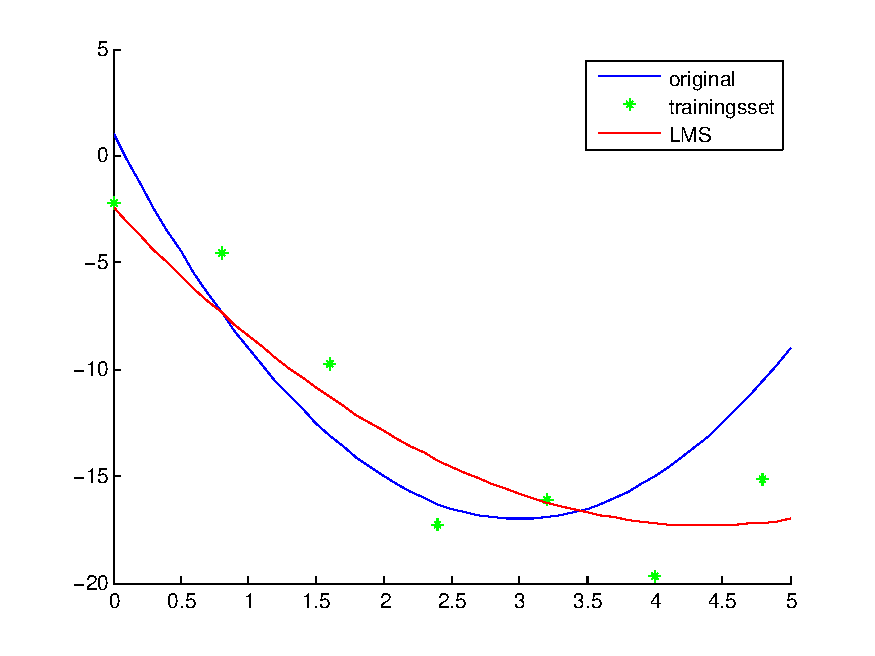
\includegraphics[width=6cm]{../figures/LMS.pdf}
	\caption{Optimization using the LMS-rule}
	\label{fig:122_LMS}
\end{figure}
The values of the resulting weight vector are summarized in Tab.~\ref{table:wLMS} and the corresponding curve plotted in Fig.~\ref{fig:122_LMS}.

\begin{itemize}
	\item How can you determine the optimal ${\mathbf w}^*$ in closed form? Compare ${\mathbf w}^*$ with the outcome of the LMS-rule training.
\end{itemize}
The closed form is calculated by updating the weight vector, determined by all N points, in one step.
\begin{itemize}	
	\item What is the influence of $\gamma$? Which value for $\gamma$ represents a good tradeoff between number of iterations and convergence? 
\end{itemize}

\subsubsection{Model-complexity and model-selection}
Determine ${\mathbf w}^*$ in closed form for 2000 different training sets, in which only the $t_i$ are varyied according to $\mathcal{N}(\mu = y_i,\sigma = 16)$, while the $x_i$ remain unchanged. 

\vspace{2mm}
\noindent {\bf Tasks}\footnote{In all tasks $\mathcal{E}$ refers to the expected value with respect to the random variable ${\mathbf w^*}$, i.e. $\mathcal{E} \equiv \mathcal{E}_{\mathbf w^*}$}:
\begin{itemize}
\item Select a fixed $x'$, which is not an observation of the training set, but lies between two observations (e.g. $x' = 2$)
\item Estimate the \emph{mean squared error} 
\begin{equation} \nonumber
\mbox{\emph{mse}} = \mathcal{E} (f(x')-f_{\mathbf w^*}(x'))^2,
\end{equation}i.e., the mean of the squared residuals of the models prediction $f_{\mathbf w^*}(x')$ from the true function value $f(x')$ for all $0 \leq d \leq 8$ ($d = 0$ corresponds to a constant function) using at least 2000 trials.  
\item Estimate by the same way the quantities \emph{bias}$^2 = (f(x')-\mathcal{E} f_{\mathbf w^*}(x'))^2$ and \emph{var}$ = (f_{\mathbf w^*}(x') - \mathcal{E} f_{\mathbf w^*}(x'))^2$.
\item Plot \emph{mse}, \emph{bias}$^2$ and \emph{var} against $d$ together in one plot. What is the relation of the quantities?
\item (optional) Generate the above plots only for $d=8$, but minimize instead of $E({\mathbf w})$ the regularized error function 
\begin{equation}
E_{\lambda}({\mathbf w}) = \sum_{i = 1}^N(t_i - {\mathbf w}^T{\mathbf \Phi}(x_i))^2 + \lambda \|{\mathbf w}\|^2,
\end{equation} 
i.e. ${\mathbf w}^* = \arg\min_{\mathbf w}^* E_{\lambda}({\mathbf w})$. Plot the quantities against $\lambda$ instead of $d$. Hint: The minimum can be obtained in closed form (see lecture slides). 
\end{itemize}

\end{document}
